\section{Our Approach}
	\label{section:app}

\subsection{Overview}
Figure~\ref{fig:overview} gives a high-level overview of our approach. To align entities from two \KGs, we first manually label some entity
pairs from the target \KGs to construct a training dataset. The training dataset contains both aligned and randomly sampled unaligned
entity pairs. Next, we extract graph information from the \KGs, which is used to capture the semantics and attributes of entities as well
as the relation of neighboring nodes (Section~\ref{section:rgcn}). Then, we learn a neural network (Section~\ref{sec:model}) to take in the
graph information (organized as matrices) and produce a representation vector for each entity of the input \KGs. The network output is
optimized in a way that two aligned entities in the training data are similar to each other in the feature space. With this entity
representation in place, we can calculate the distance between any two entity representations to determine if the entities should be
aligned (Section~\ref{prediction}).

\begin{figure}[t!]
  \centering
  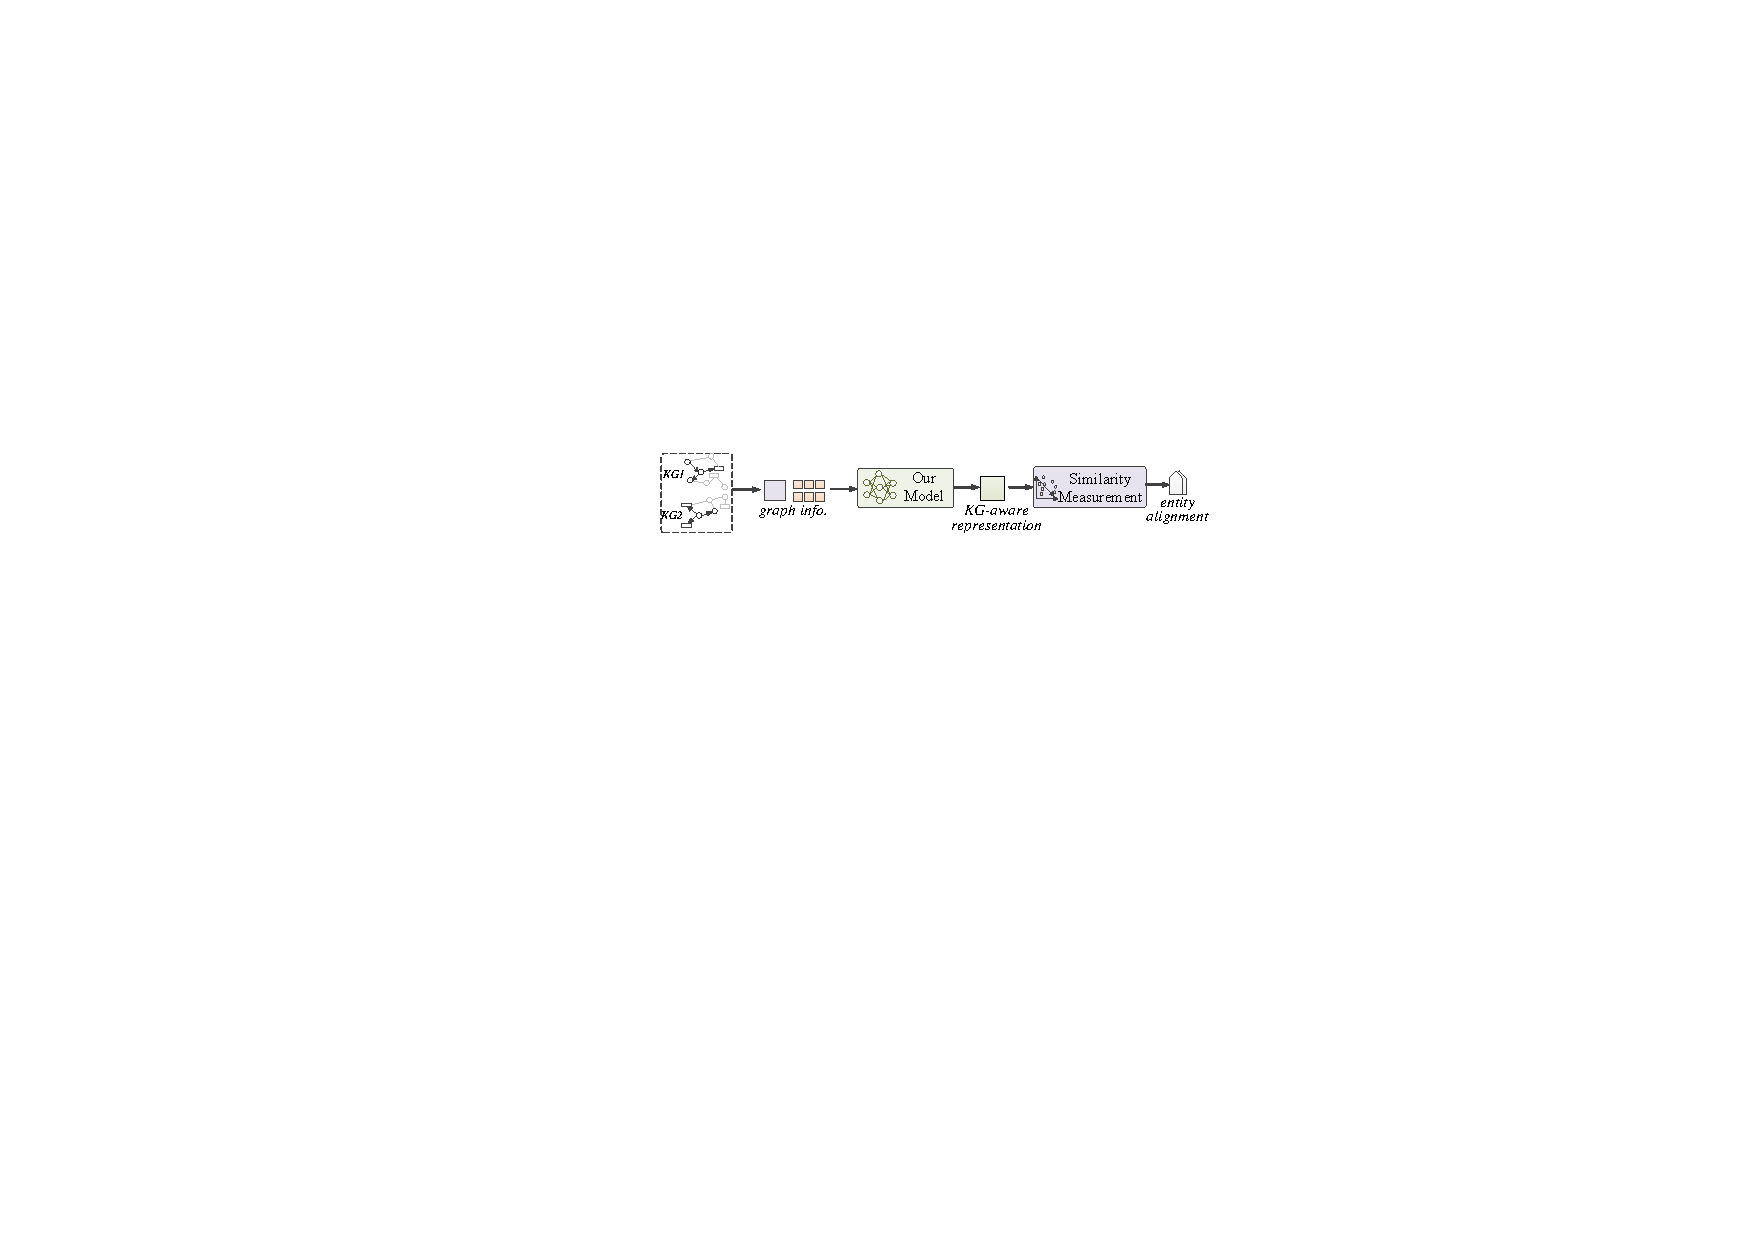
\includegraphics[width=0.5\textwidth]{figures/overview.pdf}
  \caption{Overview of our approach}\label{fig:overview}
\end{figure}


	
    \subsection{Knowledge Graph Representation Model\label{sec:model}}
    Our model for generating \KG representations  is based on the \RGCN~\cite{Schlichtkrull2017Modeling}, which is an extension of Graph Convolutional Networks (\GCNs) that operate on local graph
neighborhoods~\cite{Duvenaud2015Convolutional,Kipf2016Semi} to large-scale relational data.
   % A \RGCN layer takes a set of adjacency matrices as input, and produces a new set of node features.
%    Each input adjacency matrix describes the adjacency relationships among all nodes in the graph under each different relation.
    We choose to use the \RGCN because it can model relational (directed and labeled) multi-graphs like \KGs.

 Our work improves \RGCNs in two ways. Firstly, we use automatically learned semantic features such as entity names and attributes to
 help the \RGCN better capture the subtle correlations of entities from two different \KGs (Section~\ref{section:rgcn}.i).
    Secondly, we introduce highway gates to reduce the impact of accumulated noise when processing large graphs (Section~\ref{section:hgcn}).


 %   Our work improves the featureless approach of \RGCN with pre-defined node feature vectors.
%    We believe that in addition to the internal structures, the semantic information of entity names and the attribute information of entities can help \RGCN better embed \KGs.
%    Therefore, we incorporate the aforementioned information into the node features as part of the model inputs.


	



	
	\subsection{Knowledge Graph Information}
	\label{section:rgcn}	
  %  The input to our RGCN model are two parts. The first part is the node feature matrix $X^{(0)} \in \mathbb{R}^{N \times d^{(0)}}$ of $G$, where $N$ is the number of nodes and $d^{(0)}$ is the dimension of the input representations. We utilize predefined node features described in Section~\ref{subsection:Node Representations} to construct $X$ instead of using a featureless approach in \RGCNs~\cite{Schlichtkrull2017Modeling}.
%	The second part is the list of adjacency matrices $A=\{A_1,A_2,...,A_R |A_i \in \mathbb{R}^{N \times N} \}$, which describes the adjacency relationships among $N$ nodes under $R$ different relations. We extract $R_0$ original relations from knowledge graphs, then we add reverse relations in order to pass information from the opposite direction; and add the self loop to retain information of the node itself. These together compose $R=2R_0+1$ relations.
%	In each layer $l$, the input is $X^{(l)} = \{x^{(l)}_1,x^{(l)}_2,...,x^{(l)}_{N} |x^{(l)}_{i} \in \mathbb{R}^{d^{(l)}}\}$. The forward propagation is formulated as:
\begin{figure}
	\centering
	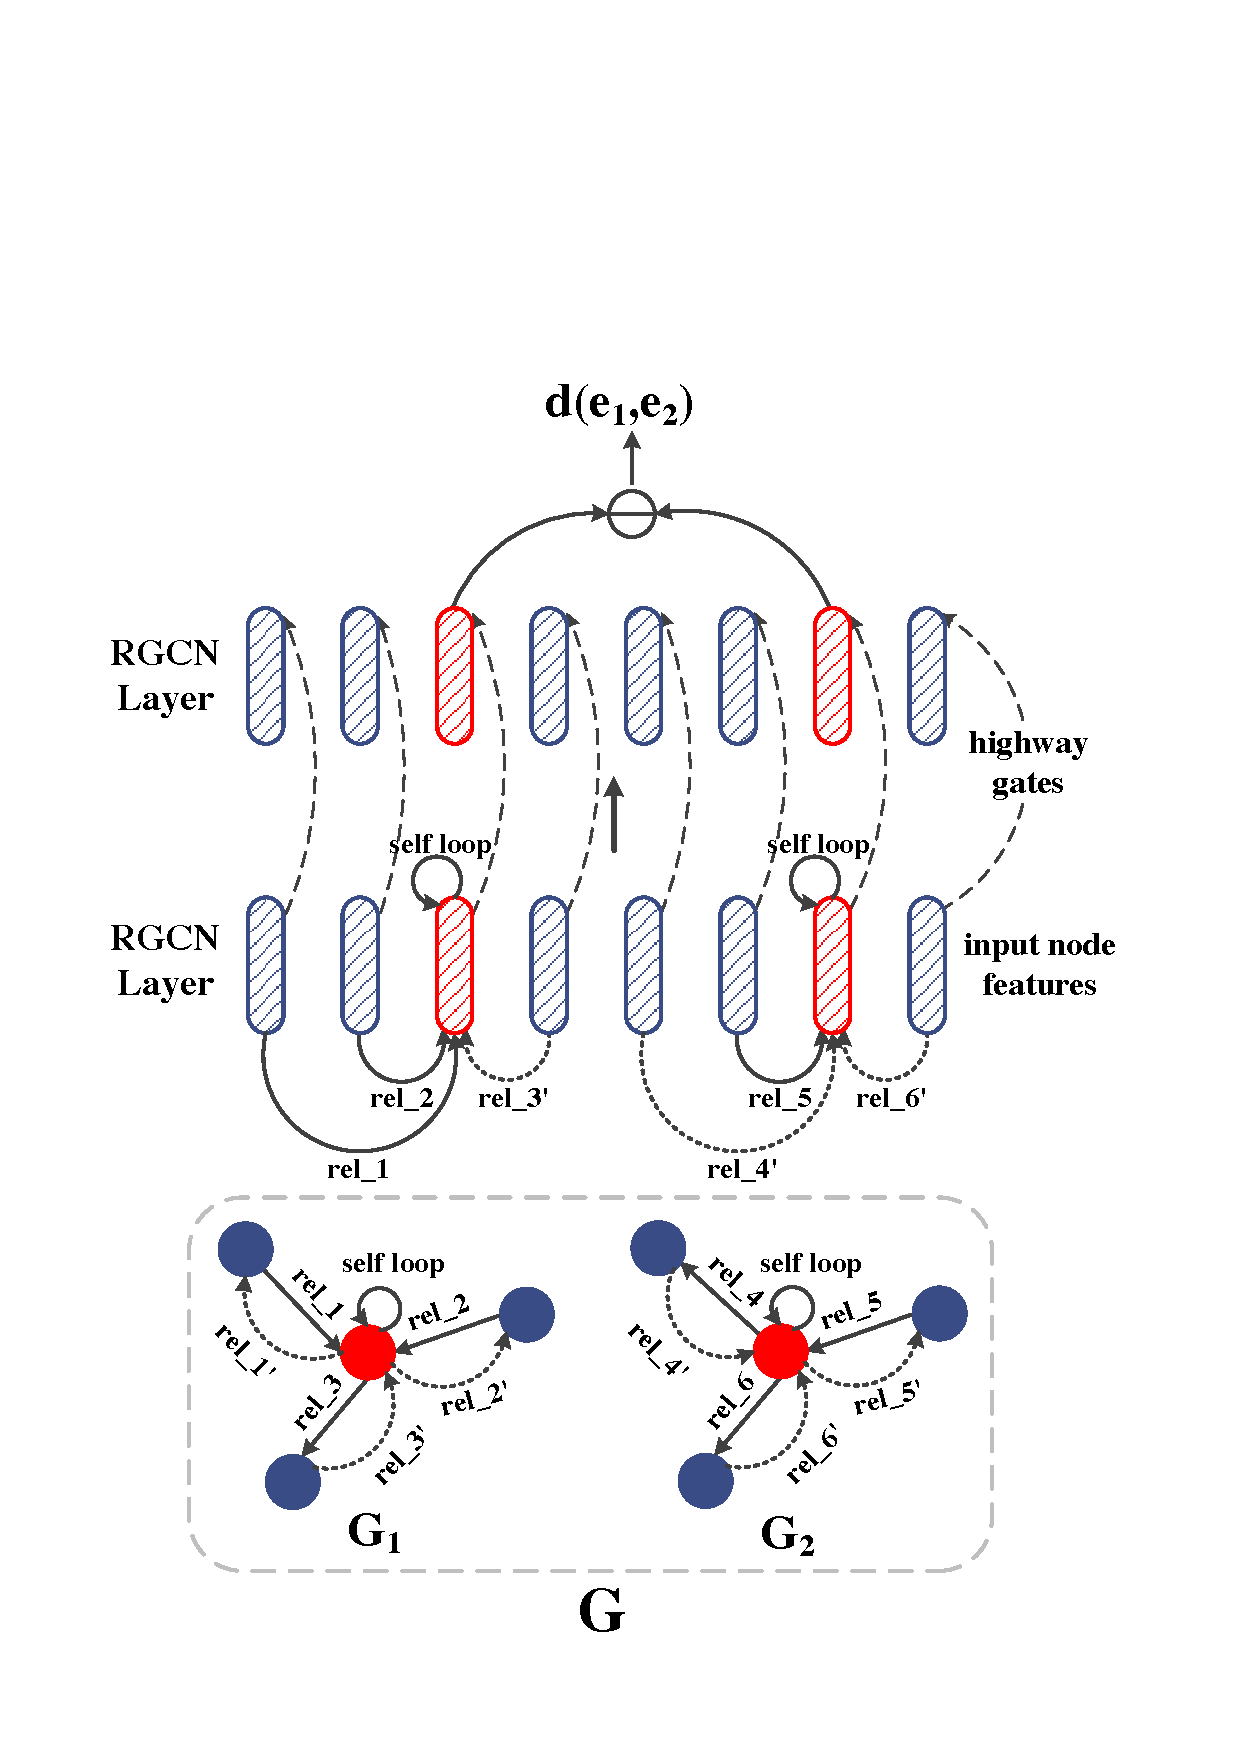
\includegraphics[width=0.4\textwidth]{figures/RGCN.pdf}
	\caption{Overall architecture of our \RGCN-based model}\label{fig:all}
\end{figure}

    Figure~\ref{fig:all} depicts the overall architecture of our \RGCN-based \KG representation model. 	
  	The input to our model consists of two parts: (i) a node feature matrix that captures the semantic information such as the entity
  names and their attributes, and (ii) a list of adjacency matrices, which describes the adjacency relationships among nodes of a \KG.
    The output of a \RGCN layer is processed by a highway gate function (Section~\ref{section:hgcn}), and the result is passed as part of
    the input to the next layer.

\subsubsection{Notations}

Without loss of generality, we introduce our model using two \KGs: $G_1 = (E_1,V_1,R_1,A_1,T_1)$ and $G_2 = (E_2,V_2,R_2,A_2,T_2)$ for
entity alignment, where $E,V,R,A,T$ represent entities, values, relations, attributes and triples respectively. 	We put $G_1$ and $G_2$
together in one large graph $G$. We utilize pre-aligned entity pairs to train our model and then discover latent aligned entities.

%


% We utilize predefined node features
% described in Section~\ref{subsection:Node Representations} to construct $X$ to capture the semantic information. 	The second part is

\subsubsection{Node representations}
	\label{subsection:Node Representations}
   We use a node feature matrix, $X \in \mathbb{R}^{N \times d}$ of $G$, to encode the semantic information of $N$  nodes in an
   input vector of $d$ elements. This representation is used to direct the \RGCN to draw attention to entity names and attributes, which are shown to be
   useful in entity alignment (Section~\ref{sec:motivation}). This node representation can be used to encode either the semantics of entity names
   or entity attributes, or a combination of both (Section~\ref{sec:combine}).


	
	\eparagraph{Encoding semantics}
	\label{wordvector}
	Intuitively, if two entities can be linked together, their names in different \KGs should have similar semantics (e.g., the \emph{XinJiang} entity in Section~\ref{sec:motivation}).
    Our work exploits this observation to improve the quality of the network features by using pre-trained word embeddings to encode the semantic
    information of entity names.
    %This is achieved by applying a word2vec model to generate word embeddings from training entity names.
    %We use an open-source word2vec implementaion\footnote{https://code.google.com/archive/p/word2vec} to generate word embeddings.

	
	\eparagraph{Encoding attributes}
    In addition to entity names, we also consider entity attributes for node representations.
	Our current implementation distinguishes four types of attributes, i.e., \emph{Integer}, \emph{Double}, \emph{Date} and \emph{String}
    (as default), but the proposed method can be extended to other data types too.
	%In this paper, we only consider the first three types, i.e., Integer, Double and Date.
%	We overlook String type values by reason of their complexity and heterogeneity in different \KGs.
%	
	For each entity in a \KG, we construct a attribute vector. The dimension of the vector equals to the number of distinct attribute values in the \KG.
    We standardize the attribute values (e.g., distances of different units are converted to meters) and pad missing attributes to form a constant-sized
    vector for each entity.

 \subsubsection{Neighboring node relation}
 Like standard \RGCNs, we capture the relation of graph neighboring nodes using an adjacency matrix.
 In our case, the adjacency matrices, $A=\{A_1,A_2,...,A_R |A_i \in \mathbb{R}^{N
 \times N} \}$, describe the adjacency relationships among $N$ nodes under $R$ different relations (i.e., edges in the \KG or predicates of entities) of graph $G$.

 To construct the adjacency matrices, $A$, we follow a number of steps. We first extract $R_0$ original
 relations from the input \KGs, then we add reverse relations in order to pass information from the opposite direction. To retain the node's
 information, we also add a self-referencing loop of a special relation type to each node. Applying these steps results in $R=2R_0+1$ relations. As shown in Figure~\ref{fig:all}, original relations, reverse relations and the self loops all participate in the updating of node features.

 \eparagraph{Calculate the embedding matrix}
 The input for layer $l$ of a \RGCN is a node feature matrix, $X^{(l)}$, of $N$ vectors, where  $X^{(l)} =\{x^{(l)}_1,x^{(l)}_2,...,x^{(l)}_{N}
 |x^{(l)}_{i} \in \mathbb{R}^{d^{(l)}}\}$. Each node feature vector, $x_i$, is updated using forward propagation as:

 %, and we stack the output vector for each node, $x_i^{(l+1)}$
% , to form an embedding matrix, $X^{(l+1)} \in \mathbb{R}^{N \times d^{(l+1)}}$.
	\begin{equation}
	x_i^{(l+1)}=\mathrm{ReLU} (\sum\limits_{r \in R}\sum\limits_{j \in N_i^r}\frac{1}{|N_i^r|}W_r^{(l)}x_j^{(l)}),
	\end{equation} where $N_i^r$ is the set of neighbor indices of node $i$ under relation $r$.
    $N_i^r$ is computed based on the normalized adjacency
matrix $\hat A_r$ -- an approximate of spectral convolutions on the adjacency matrix $A_r$~\cite{Kipf2016Semi}:
	\begin{equation}
	\hat A_r=\hat D_r^{- \frac{1}{2}}(A_r+I)\hat D_r^{- \frac{1}{2}},
	\end{equation}
	where $(\hat D_r)_{jj}=\sum_k(A_r+I)_{jk}$, and $I$ is an identity matrix.

	
	\eparagraph{Calculate the weight matrix} For each relation $r$, we construct a weight matrix, $W_r^{(l)} \in \mathbb{R}^{d^{(l+1)}
\times d^{(l)}}$. As a \KG often has over thousands of types of relations, there will be a large amount of network parameters to learn
over, making the trained model more likely to overfit. To minimize the impact of the parameter size, we employ the basis decomposition
method~\cite{Schlichtkrull2017Modeling} to regularize the weights:
	\begin{equation}
	W_r^{(l)}=\sum\limits_{b=1}^B a_{rb}^{(l)}V_b^{(l)},
	\end{equation}
	where $V_b^{(l)} \in \mathbb{R}^{d^{(l+1)} \times d^{(l)}}$ and $a_{rb}^{(l)}$ is the coefficient of matrix $V_b^{(l)}$ for relation $r$.
	
	
%	Since it is the first attempt, we only consider the numerical part of a value, regardless of the unit, that is, we do not insist on normalizing \emph{1.80m} and \emph{180cm}.
%	We leave this for future work.


	\subsection{Noise Control Through Highway Gates}
	\label{section:hgcn}
%	While stacking \RGCN layers enhances our model's capability in learning neighborhood information from relational steps, it may as well
%bring noise from the exponentially increasing number of neighbors.
One of the challenges for applying \GCNs to a large \KG is that the noise accumulated across network layers can have a seriously negative
impact on the learning quality. To tackle this challenge, we employ layer-wise gates similar to highway
networks~\cite{Srivastava2015Highway} to process the output of the \RGCN. This results in a novel highway \RGCN for entity alignment, for
which we refer as \HRGCN thereafter. With highway gates, the output of a \HRGCN layer is computed as:
%
%
% To ensure effective spread of informative and discriminative neighborhood information, we add layer-wise gates
%similar to highway networks~\cite{Srivastava2015Highway} to our \RGCN-based model.
%%~\cite{Rahimi2018Semi} have successfully introduced highway gates to \GCNs~\cite{Kipf2016Semi} to solve the user geolocation problem.
%We use layer-wise highway gates to build a Highway \RGCN (\HRGCN) model where the output of a \HRGCN layer is computed as:
	\begin{equation}
	\begin{split}
	&T(x^{(l)})=\sigma(W_T^{(l)}x^{(l)}+b_T^{(l)}), \\
	&x^{(l+1)}=x^{(l+1)} \cdot T(x^{(l)})+x^{(l)} \cdot (1-T(x^{(l)})),
	\end{split}
	\end{equation}
	where $\sigma$ is a sigmoid activation function, $\cdot$ is element-wise multiplication, $W_T^{(l)} \in \mathbb{R}^{d^{(l+1)} \times
d^{(l)}}$ and $b_T^{(l)} \in \mathbb{R}^{d^{(l)} \times 1}$ are the weight matrix and bias vector of highway gate $T(x^{(l)})$,
respectively.


\subsection{Exploiting Entity Semantics and Attributes\label{sec:combine}}
    Recall that the node feature vector can be constructed from either entity name semantics or entity attributes (Section~\ref{subsection:Node
    Representations}). There are multiple ways to exploit the semantic and attribute embeddings. One is to simply concatenate a pre-trained word vector
    and an attribute vector as an input node feature vector. Another is to apply two stacked \HRGCNs to respectively perform a
    semantic or an attribute embedding.  We provide a further discussion on these strategies in Section~\ref{sec:analysis}.

    For stacked \HRGCNs, we define a new feature vector, $d$, to combine the semantic and attribute embeddings produced by each \HRGCN:
	\begin{equation}
		d(e_1,e_2)=\frac{1}{m}[\omega d_s(e_1,e_2)+(1-\omega)d_a(e_1,e_2)]
	\end{equation}

	where $m$ is the dimension of the new node features produced by \HRGCNs, $\omega$ is a hyper-parameter, and $d_s$ and $d_a$ are the distance computed by Eq.~\ref{d} according to semantic and attribute embeddings, respectively.
	
	\subsection{Entity Alignment Prediction and Training\label{prediction}}
   In our work, entity alignment is based on the network output's (i.e., the graph representation), $\bar{X}$ -- an embedding matrix of $N$ vectors, $\bar{x}_1,\bar{x}_2,...,\bar{x}_N$, where
   each vector, $\bar{x}$, corresponds to one
    of the $N$ entity nodes within graph $G$. 	


\cparagraph{Alignment} With the graph representation in place, entity alignment is as simple as measuring the similarity between two entity
nodes in the representation space. Specifically, the similarity, $d(e_1,e_2)$, between two entity nodes, $e_1$ from \texttt{KG1} and $e_2$
from \texttt{KG2} is calculated as:
	\begin{equation}
	\label{d}
	d(e_1,e_2)=||\bar{x}_{e_1}-\bar{x}_{e_2}||_{L_1}.
	\end{equation}

	\cparagraph{Training objective} Since we expect the distance for latent aligned entities to be smaller than the non-equivalent counterparts and hope the distance
between positive and negative aligned entity pairs can be separated by a large margin, we utilize a margin-based score function as the
training objective, defined as:
	\begin{equation}
	L=\sum\limits_{(p,q)\in \mathbb{L}}\sum\limits_{(p',q')\in \mathbb{L'}}\mathrm{max}\{0,d(p,q)-d(p',q')+\gamma\},
	\end{equation}
	where $\gamma > 0$ is a margin hyper-parameter; $\mathbb{L'}$ stands for the negative alignment set of $\mathbb{L}$, defined as follows:
	\begin{equation}
	\mathbb{L'}=\{(p',q)|p'\in E_1\}\cup\{(p,q')|q'\in E_2\}, (p,q)\in \mathbb{L'}.
	\end{equation}
	This indicates one of two entities in an aligned entity pair is randomly replaced by others.
	
	%In our experiments, for a entity $e_1$ in $G_1$, we compute the distances between $e_1$ and all the entities in $G_2$. The alignment process can also be reversed, i.e., from $G_2$ to $G_1$. In Section~\ref{sec:results}, we report the results of both directions of entity alignment.

	
	

	%In our experiments, we set the output dimensions of two models (one for semantic embedding and the other one for attribute embedding) to be the same.
	
	
